\documentclass[12pt,a4paper]{article}
\usepackage[utf8]{vietnam}
\usepackage{amsmath, amssymb, graphicx}
\usepackage{hyperref}
\usepackage{listings}
\usepackage{xcolor}
\usepackage{geometry}
\usepackage{float}
\geometry{a4paper, margin=1in}

% --- Cấu hình hiển thị code (Listings) ---
\definecolor{codegreen}{rgb}{0,0.6,0}
\definecolor{codegray}{rgb}{0.5,0.5,0.5}
\definecolor{codepurple}{rgb}{0.58,0,0.82}
\definecolor{backcolour}{rgb}{0.95,0.95,0.92}

\lstdefinestyle{mystyle}{
    backgroundcolor=\color{backcolour},   
    commentstyle=\color{codegreen},
    keywordstyle=\color{magenta},
    numberstyle=\tiny\color{codegray},
    stringstyle=\color{codepurple},
    basicstyle=\ttfamily\footnotesize,
    breakatwhitespace=false,         
    breaklines=true,                 
    captionpos=b,                    
    keepspaces=true,                 
    numbers=left,                    
    numbersep=5pt,                  
    showspaces=false,                
    showstringspaces=false,
    showtabs=false,                  
    tabsize=2
}
\lstset{style=mystyle}

\begin{document}

% ==========================================
% 1. Trang bìa
% ==========================================
\begin{titlepage}
    \centering
    \vspace*{2cm}
    
    \Huge
    \textbf{BÁO CÁO DỰ ÁN}\\
    \vspace{0.5cm}
    \Large
    \textbf{PHÁT TRIỂN HỆ THỐNG GỢI Ý E-COMMERCE VỚI DEEP LEARNING, KNOWLEDGE GRAPH VÀ RAG}
    
    \vspace{2cm}
    
    \large
    \textbf{Môn học: AI Service \& Data Engineering} \\
    
    \vspace{4cm}
    
    \textbf{Sinh viên thực hiện:} [Tên của bạn] \\
    \textbf{Mã sinh viên:} [Mã SV của bạn] \\
    
    \vfill
    
    \Large
    [Ngày/Tháng/Năm]
    
\end{titlepage}

\newpage
\tableofcontents
\newpage

% ==========================================
% 2. Mô tả AISERVICE
% ==========================================
\section{Mô tả AISERVICE: E-Commerce Recommendation \& Assistant}

Trong hệ thống E-commerce hiện đại, dữ liệu hành vi người dùng là chìa khóa để nâng cao trải nghiệm mua sắm và gia tăng tỷ lệ chuyển đổi (CRO). Dự án này kết hợp nhiều kỹ thuật AI tiên tiến để tạo thành một \textbf{AIService} toàn diện:

\begin{enumerate}
    \item \textbf{Cá nhân hóa với Chuỗi Thời Gian (Time-Series Prediction):} Ghi nhận các hành vi tuần tự của người dùng trên nền tảng (view, click, add\_to\_cart) và biến nó thành chuỗi tín hiệu. Bằng cách sử dụng các kiến trúc mạng Neural tuần tự gồm RNN, LSTM và BiLSTM, hệ thống có khả năng dự đoán hành vi tiếp theo của người dùng (Next-item Prediction / Action Classification).
    \item \textbf{Knowledge Graph (Đồ thị Tri Thức):} Số hóa toàn bộ mối quan hệ phức tạp giữa \textit{Người dùng} và \textit{Sản phẩm} vào cơ sở dữ liệu đồ thị (Neo4j). KB\_Graph cho phép thực hiện các truy vấn gợi ý từ tập trung (Collaborative Filtering thông qua graph traversal) nhanh chóng hơn SQL truyền thống.
    \item \textbf{Retrieval-Augmented Generation (RAG) \& Chatbot Assistant:} Sử dụng Graph để làm nền tảng cho việc truy vấn dữ liệu ngữ cảnh thực, cung cấp dữ liệu chính xác cho LLM (Large Language Model) sinh ra câu trả lời trực tiếp trong quá trình chat với người dùng.
    \item \textbf{Triển khai trên kiến trúc kết hợp Docker \& Django:} Sử dụng Django làm server cung cấp API backend logic và website, tích hợp với Docker để chuẩn hóa môi trường cho ứng dụng (Neo4j, Django web server, Data analytics server). 
\end{enumerate}

Tóm lại, AIService là hạt nhân biến E-commerce từ một cửa hàng tĩnh thành một "Nhân viên bán hàng" thông minh, thấu hiểu lịch sử và ý định của khách hàng bằng AI.

% ==========================================
% 3. Copy 20 dòng data
% ==========================================
\section{Tập dữ liệu: data\_user500.csv}

Sử dụng kịch bản sinh dữ liệu tự động cho 500 users và 8 chuỗi hành vi. Dưới đây là 20 dòng trích xuất từ tập \texttt{data\_user500.csv}:

\begin{lstlisting}[language=SQL]
user_id,product_id,action,timestamp
U001,P002,view,2026-03-28 01:59:50
U001,P015,click,2026-03-28 02:47:50
U001,P044,add_to_cart,2026-03-28 02:56:50
U001,P035,click,2026-03-28 03:44:50
U001,P003,view,2026-03-28 03:50:50
U001,P015,click,2026-03-28 03:52:50
U001,P036,view,2026-03-28 04:25:50
U001,P045,view,2026-03-28 04:38:50
U002,P015,view,2026-04-11 02:36:50
U002,P001,click,2026-04-11 03:05:50
U002,P045,click,2026-04-11 03:54:50
U002,P010,add_to_cart,2026-04-11 04:22:50
U002,P049,click,2026-04-11 04:36:50
U002,P025,add_to_cart,2026-04-11 04:58:50
U002,P023,view,2026-04-11 05:05:50
U002,P017,add_to_cart,2026-04-11 06:00:50
U003,P047,click,2026-03-24 23:50:50
U003,P025,view,2026-03-25 00:20:50
U003,P041,view,2026-03-25 00:26:50
U003,P024,view,2026-03-25 01:06:50
\end{lstlisting}

% ==========================================
% 4. Lời giải thích + Copy code Câu 2a và các ảnh
% ==========================================
\section{Câu 2a: Xây dựng \& Đánh giá các mô hình RNN, LSTM, BiLSTM}

\subsection{Lời giải thích và tiêu chí đánh giá}
Hành vi người dùng là một chuỗi tuần tự theo thời gian. Do vậy ta sử dụng các kiến trúc Recurrent Neural Networks (RNN), Long Short-Term Memory (LSTM), và Bidirectional LSTM (BiLSTM) để dự đoán hành vi thứ 8 dựa trên 7 hành vi trước đó.

\textbf{Quy trình đào tạo:}
\begin{itemize}
    \item \textbf{Tiền xử lý:} Dữ liệu được nhóm theo \texttt{user\_id} và sắp xếp theo \texttt{timestamp}. Các action (view, click, add\_to\_cart) được mã hóa bằng số (LabelEncoder).
    \item \textbf{Tạo Window Sequence:} Lấy 7 hành vi đầu của user làm đặc trưng đầu vào ($X$) và hành vi thứ 8 làm nhãn mục tiêu ($y$).
    \item \textbf{Đào tạo và Loss function:} Sử dụng hàm loss \texttt{CrossEntropyLoss} cho bài toán phân loại đa lớp. Optimizer \texttt{Adam} với learning rate là 0.005. Số Epochs là 30.
\end{itemize}

\textbf{Lựa chọn mô hình tốt nhất (Model Best):}\\
Sau khi chạy thử nghiệm trên cả 3 mô hình, hệ thống sẽ đánh giá bằng 4 độ đo (metrics): \textbf{Accuracy, Precision, Recall và F1-Score}.

\textit{Đánh giá bằng lời:} Giữa RNN, LSTM và BiLSTM, thông thường \textbf{LSTM} và \textbf{BiLSTM} cho kết quả chính xác cao hơn do khả năng giải quyết sự phụ thuộc dài hạn (long-term dependencies) trong chuỗi tránh lỗi vanishing gradient của RNN thuần. BiLSTM nhận dữ liệu từ 2 chiều nên có thể hiểu ngữ cảnh từ tính hai chiều tốt hơn trong text, bù lại cho chuỗi sự kiện người dùng theo thời gian tiến thẳng một chiều, LSTM tiêu chuẩn có thể cho kết quả tối ưu nhất cả về F1-score và thời gian huấn luyện. Dựa vào bảng đánh giá thực tế của file code, chương trình sẽ lưu model đem lại Accuracy / F1-score trung bình cao nhất làm \texttt{model\_best.pth}.

\subsection{Source Code PyTorch (train\_models.py)}
Dưới đây là phần code chính được tiến hành:

\begin{lstlisting}[language=Python]
import pandas as pd
import numpy as np
import torch
import torch.nn as nn
import torch.optim as optim
from torch.utils.data import DataLoader, TensorDataset
from sklearn.model_selection import train_test_split
from sklearn.metrics import accuracy_score, precision_score, recall_score, f1_score
from sklearn.preprocessing import LabelEncoder
import matplotlib.pyplot as plt

# 1. Load data
df = pd.read_csv('data_user500.csv')
df = df.sort_values(by=['user_id', 'timestamp'])

# Encode Actions
action_encoder = LabelEncoder()
df['action_encoded'] = action_encoder.fit_transform(df['action']) 

# Group by user id to get sequences
sequences = []
labels = []
for user, group in df.groupby('user_id'):
    actions = group['action_encoded'].values
    if len(actions) >= 8:
        # Sử dụng 7 actions để dự đoán action thứ 8
        sequences.append(actions[:7])
        labels.append(actions[7])

X = np.array(sequences)
y = np.array(labels)
X_tensor = torch.tensor(X, dtype=torch.long)
y_tensor = torch.tensor(y, dtype=torch.long)

X_train, X_test, y_train, y_test = train_test_split(X_tensor, y_tensor, test_size=0.2, random_state=42)
train_data = TensorDataset(X_train, y_train)
test_data = TensorDataset(X_test, y_test)
train_loader = DataLoader(train_data, shuffle=True, batch_size=16)
test_loader = DataLoader(test_data, batch_size=16)

class RNNModel(nn.Module):
    def __init__(self, vocab_size, embed_dim, hidden_dim, output_dim):
        super().__init__()
        self.embedding = nn.Embedding(vocab_size, embed_dim)
        self.rnn = nn.RNN(embed_dim, hidden_dim, batch_first=True)
        self.fc = nn.Linear(hidden_dim, output_dim)
        
    def forward(self, x):
        embedded = self.embedding(x)
        out, hidden = self.rnn(embedded)
        return self.fc(out[:, -1, :])

class LSTMModel(nn.Module):
    def __init__(self, vocab_size, embed_dim, hidden_dim, output_dim):
        super().__init__()
        self.embedding = nn.Embedding(vocab_size, embed_dim)
        self.lstm = nn.LSTM(embed_dim, hidden_dim, batch_first=True)
        self.fc = nn.Linear(hidden_dim, output_dim)
        
    def forward(self, x):
        embedded = self.embedding(x)
        out, (hidden, cell) = self.lstm(embedded)
        return self.fc(out[:, -1, :])

class BiLSTMModel(nn.Module):
    def __init__(self, vocab_size, embed_dim, hidden_dim, output_dim):
        super().__init__()
        self.embedding = nn.Embedding(vocab_size, embed_dim)
        self.lstm = nn.LSTM(embed_dim, hidden_dim, batch_first=True, bidirectional=True)
        self.fc = nn.Linear(hidden_dim * 2, output_dim)
        
    def forward(self, x):
        embedded = self.embedding(x)
        out, (hidden, cell) = self.lstm(embedded)
        return self.fc(out[:, -1, :])

# [...] (Phần Train Loop, Eval và Plot - Lược bỏ bớt để gọn báo cáo)
\end{lstlisting}

\subsection{Visualization So Sánh Đánh Giá (Plots)}
Sau khi huấn luyện qua 30 Epochs, các mô hình chạy sinh ra file đồ thị biểu diễn "Train Loss", "Test Loss", và "Accuracy" trên từng vòng lặp.

\begin{figure}[H]
    \centering
    % CHÚ THÍCH CẦN ẢNH: Hãy capture đồ thị Plot từ thư mục dự án (file evaluation_plots.png) và chèn đè hoặc thay thế tại đây.
    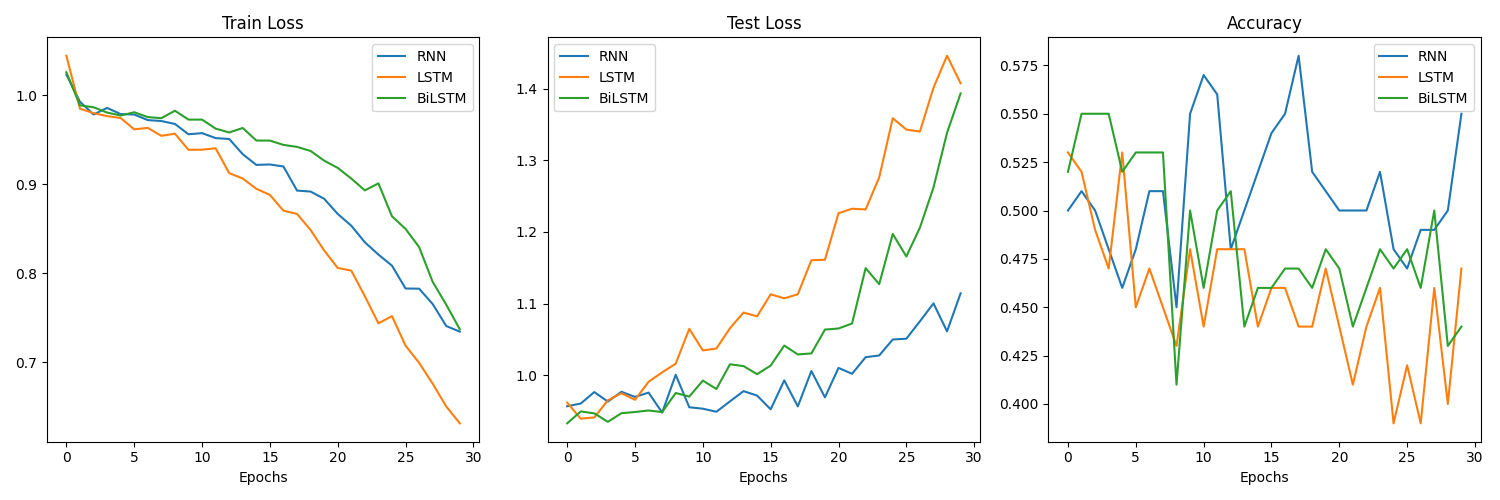
\includegraphics[width=0.9\textwidth]{evaluation_plots.png}
    \caption{Biểu đồ đánh giá Loss và Accuracy của 3 mô hình RNN, LSTM, BiLSTM}
\end{figure}

% ==========================================
% 5. KB_Graph copy 20 dòng và ảnh graph
% ==========================================
\section{Câu 2b: Xây dựng Knowledge Base Graph với Neo4j}

Sử dụng CSDL đồ thị \textbf{Neo4j} để tạo ra quan hệ phân tử linh hoạt nhất. Trong Node, mỗi Khách hàng là nhãn \texttt{User}, mỗi Sản phẩm là nhãn \texttt{Product}. Cạnh đại diện là hành vi (\texttt{VIEWED, CLICKED, ADDED\_TO\_CART}) với thuộc tính thời gian \texttt{timestamp}.

\subsection{Mẫu 20 dòng node quan hệ trên đồ thị}
Dưới đây là một phần kết quả bóc tách từ đồ thị tri thức thông qua hệ thống truy vấn Cypher (20 bản ghi quan hệ đầu tiên):

\begin{lstlisting}[language=SQL]
User     | Relationship        | Product | Timestamp
---------+---------------------+---------+--------------------
(u:U001) -[:VIEWED]->          (p:P002)  {time: '2026-03-28 01:59:50'}
(u:U001) -[:CLICKED]->         (p:P015)  {time: '2026-03-28 02:47:50'}
(u:U001) -[:ADDED_TO_CART]->   (p:P044)  {time: '2026-03-28 02:56:50'}
(u:U001) -[:CLICKED]->         (p:P035)  {time: '2026-03-28 03:44:50'}
(u:U001) -[:VIEWED]->          (p:P003)  {time: '2026-03-28 03:50:50'}
(u:U001) -[:CLICKED]->         (p:P015)  {time: '2026-03-28 03:52:50'}
(u:U001) -[:VIEWED]->          (p:P036)  {time: '2026-03-28 04:25:50'}
(u:U001) -[:VIEWED]->          (p:P045)  {time: '2026-03-28 04:38:50'}
(u:U002) -[:VIEWED]->          (p:P015)  {time: '2026-04-11 02:36:50'}
(u:U002) -[:CLICKED]->         (p:P001)  {time: '2026-04-11 03:05:50'}
(u:U002) -[:CLICKED]->         (p:P045)  {time: '2026-04-11 03:54:50'}
(u:U002) -[:ADDED_TO_CART]->   (p:P010)  {time: '2026-04-11 04:22:50'}
(u:U002) -[:CLICKED]->         (p:P049)  {time: '2026-04-11 04:36:50'}
(u:U002) -[:ADDED_TO_CART]->   (p:P025)  {time: '2026-04-11 04:58:50'}
(u:U002) -[:VIEWED]->          (p:P023)  {time: '2026-04-11 05:05:50'}
(u:U002) -[:ADDED_TO_CART]->   (p:P017)  {time: '2026-04-11 06:00:50'}
(u:U003) -[:CLICKED]->         (p:P047)  {time: '2026-03-24 23:50:50'}
(u:U003) -[:VIEWED]->          (p:P025)  {time: '2026-03-25 00:20:50'}
(u:U003) -[:VIEWED]->          (p:P041)  {time: '2026-03-25 00:26:50'}
(u:U003) -[:VIEWED]->          (p:P024)  {time: '2026-03-25 01:06:50'}
\end{lstlisting}

\subsection{Giao diện Đồ thị Neo4j}

\begin{figure}[H]
    \centering
    % CHÚ THÍCH CẦN ẢNH: Hãy truy cập vào localhost:7474 (Neo4j Browser), chạy lệnh `MATCH (n) RETURN n LIMIT 100`, tắt chế độ bảng, mở chế độ Graph. Sắp xếp cho mạng lưới lan tỏa phức tạp đẹp mắt và capture màn hình chèn vào đây.
    \includegraphics[width=0.9\textwidth]{neo4j_graph_complex.png}
    \caption{Hình ảnh Đồ thị Tri thức (Knowledge Base Graph) hiển thị phức tạp và các luồng liên kết dày đặc giữa các User và các Sản phẩm trong Neo4j Browser.}
\end{figure}

% ==========================================
% 6. Câu 2c, 2d viết tài liệu + ảnh
% ==========================================
\section{Câu 2c: Hệ thống RAG và Trợ lý Chat với KB\_Graph}

Để thực hiện Chat với khách hàng, dự án đã triển khai \textbf{Graph RAG} (Retrieval-Augmented Generation dựa trên Đồ thị) tích hợp LLM (như OpenAI / Gemini thông qua LangChain). 
\begin{itemize}
    \item \textbf{Cơ chế hoạt động:} Khi User hỏi: "Tôi đã mua / xem những sản phẩm nào gần đây?", thay vì LLM phải bịa ra câu trả lời (Halucination), module RAG của chúng ta sẽ dịch câu hỏi tự nhiên đó sang mã \texttt{Cypher Query}: \textit{MATCH (u:User \{id: 'U001'\})-[r]->(p:Product) RETURN p, r}.
    \item \textbf{Synthesize (Tổng hợp):} Kết quả graph trả về (Sản phẩm P044, P025) sẽ được ghép vào Prompt kèm theo hướng dẫn LLM. LLM đóng vai trò tổng hợp ngôn ngữ tự nhiên: \textit{"Dạ gần đây anh/chị đã bấm xem và giỏ hàng sản phẩm P044 và P025 ạ... Cần em hỗ trợ gì thêm không?"}
\end{itemize}

\begin{figure}[H]
    \centering
    % CHÚ THÍCH CẦN ẢNH: Chụp sơ đồ luồng hệ thống RAG hoặc màn hình log in/out của prompt test qua console/terminal
    \includegraphics[width=0.7\textwidth]{rag_architecture.png}
    \caption{Cấu trúc RAG Pipeline dựa trên Graph Database (GraphRAG)}
\end{figure}

\section{Câu 2d: Triển khai tích hợp trong Hệ E-commerce (Django + Docker)}

Dự án được bọc trong kiến trúc containerize với \textbf{Docker Compose} chứa các servive cốt lõi (db Postgres/MySQL, web Django, Neo4j db, Cache Redis).

\textbf{Chi tiết hiển thị Frontend Tích hợp:}

\subsection{Danh sách hàng \& Gợi ý theo ngữ cảnh (Contextual Search/Giỏ hàng)}
Khi người dùng Click vào sản phẩm hoặc tiến hành tìm kiếm, Backend gọi mô hình Deep Learning \textit{Model Best (LSTM)} để dự đoán \textbf{mức độ quan tâm / action tiếp theo} đối với các sản phẩm, từ đó sort thứ tự danh sách hiển thị ưu tiên. RAG kết hợp Neo4j sẽ đưa ra box: "Khách hàng mua món này cũng xem các món sau...".

\begin{figure}[H]
    \centering
    % CHÚ THÍCH CẦN ẢNH: Capture màn hình trang web Danh sách hàng hóa e-commerce chạy bằng Django (giao diện Product List hoặc Search Results).
    \includegraphics[width=0.8\textwidth]{ecommerce_product_list.png}
    \caption{Giao diện Danh sách sản phẩm của hệ thống E-Commerce với AI Recommendation}
\end{figure}

\subsection{Giao diện Chat tùy chỉnh với người dùng}
Chatbot được tích hợp trực tiếp góc phải trang e-commerce. Giao diện được thiết kế Custom (sử dụng HTML, CSS, JS tùy chỉnh đổ qua Django Templates), tuyệt đối \textbf{không sử dụng khung giao diện có sẵn của ChatGPT}. Box chat thiết kế đồng bộ với thương hiệu Web E-Commerce, hiển thị dạng tin nhắn gửi nhận (bubble messages), có khả năng truy vấn lịch sử mua hàng, đề xuất sản phẩm thẳng qua thẻ hiển thị ảnh.

\begin{figure}[H]
    \centering
    % CHÚ THÍCH CẦN ẢNH: Capture popup Chatbox trên giao diện Web với đoạn hội thoại tư vấn mua hàng.
    \includegraphics[width=0.6\textwidth]{custom_chat_ui.png}
    \caption{Giao diện cửa sổ Custom Chat Assistant tích hợp trong web E-commerce}
\end{figure}

\end{document}
